\subsection*{\Large Общая характеристика работы}
\fontsize{14pt}{15pt}\selectfont
\textbf{Актуальность темы.}
Визуальное моделирование --- это подход к разработке программного обеспечения (ПО), в котором программа представляется 
в виде набора графических моделей, каждая из которых описывает её с разных точек 
зрения. Благодаря наличию стандартных широко распространённых графических языков, 
визуальное моделирование повышает продуктивность разработки ПО и качество результирующего 
продукта. При этом по набору визуальных моделей возможно автоматически генерировать программы 
целиком или их фрагменты, тем самым переиспользуя результаты анализа и проектирования.

Использование визуальных языков общего назначения, таких как UML, без заранее 
подготовленного набора библиотек и генераторов, делает задачу разработки 
программного обеспечения недостаточно эффективной в силу наличия семантического разрыва между 
кодом и моделями. Такие языки оперируют теми же терминами, что и традиционные текстовые языки 
(классы, объекты, компоненты и т.д.), поэтому, чтобы полностью специфицировать 
поведение системы и сделать возможной автоматическую генерацию, модель должна 
содержать в себе столько же информации, что и исходный код программы, но это 
противоречит самому понятию модели как некоего упрощения моделируемого объекта. 
На самом деле, визуальная модель в этом случае даже менее удобна, чем код 
программы --- визуальные символы занимают на экране больше места, чем текст. 
Если же визуальная модель будет изображать только важные аспекты 
функционирования системы, опуская излишние подробности, то она будет обозрима и полезна 
для человека, но это сделает её бесполезной для исполнителя (например, для интерпретатора или генератора исходного кода). 
Поэтому UML в основном сейчас используется как средство для анализа и 
дизайна системы, а сама система программируется на текстовых языках. Большинство инструментов 
для создания UML-диаграмм позволяют генерировать заглушки, куда предполагается дописывать код вручную, но 
существенного выигрыша для разработчиков это не даёт. Наличие заранее подготовленных 
библиотек, шаблонов и генераторов кода может существенно улучшить ситуацию, но подобные 
технологии оказываются применимы только для той предметной области, для которой они создавались.

Существует принципиально другой подход к использованию визуального 
моделирования, называемый предметно-ориентированным моделированием. Он основан на том наблюдении, что часто создать новый 
язык для узкой предметной области или даже для конкретной задачи и решить задачу 
на нём оказывается быстрее и эффективнее, чем решать эту задачу на языке общего назначения. 
В таком случае наличие знаний о предметной области позволяет добиться полной автоматической генерации программ по визуальным моделям.
Ряд исследований (проводимых, в частности, S. Kelly, R. Kieburtz) показывает, что продуктивность 
труда программистов при использовании предметно-ориентированных языков вырастает в 3-10 раз по сравнению с 
использованием языков общего назначения, поэтому такой подход представляется 
весьма перспективным.

Разумеется, создавать новый предметно-ориентированный визуальный язык и 
инструментальные средства его поддержки <<с нуля>> для каждой узкой предметной 
области или конкретной задачи было бы неоправданно трудозатратно. Поэтому 
существуют специальные средства для автоматизации этой задачи, называемые 
DSM-платформами или MetaCASE-средствами. Такие средства позволяют задать 
синтаксис визуального языка, используя какой-либо формализм (как правило, 
это метамодели), и автоматически сгенерировать редактор для этого языка и другие средства инструментальной 
поддержки (мы будем называть результат генерации DSM-решением). 
Это позволяет реализовывать технологии программирования, использующие новые предметно-ориентированные языки, в рамках приемлемых трудозатрат, 
что позволяет применять предметно-ориентированное моделирование даже для небольших проектов. Существуют зрелые исследовательские и промышленные 
DSM-платформы, такие как Eclipse Modeling Project, MetaEdit+ и другие. Однако 
несмотря на преимущества предметно-ориентированного моделирования, применяется оно 
довольно редко. Во многих случаях для создания предметно-ориентированного 
решения требуется привлекать экспертов в разработке языков моделирования, которыми зачастую 
оказываются авторы выбранной для реализации этого решения DSM-платформы, что могут
позволить себе лишь крупные компании. Такая ситуация указывает на 
необходимость продолжения исследований в этой области с целью упростить процесс создания
предметно-ориентированных решений и снизить требования к квалификации специалистов, 
которые могли бы этим заниматься.

\textbf{Степень разработанности темы.}
Методические вопросы создания предметно-ориентированных языков хорошо проработаны в случае, если 
языки текстовые (заслуживают упоминания работы A. Van Deursen, M. Mernik), для визуальных
языков сейчас существует лишь набор слабо структурированных рекомендаций и наблюдений
(наиболее обстоятельно этим вопросом занималась исследовательская группа во главе 
со S. Kelly и J.-P. Tolvanen, заслуживают упоминания работы M. Voelter). Тем не менее, 
существует довольно много DSM-платформ, многие из которых хорошо описаны в литературе 
(MetaEdit+, Eclipse Modeling Project, Generic Modeling Environment, PSL/PSA, AToM\textsuperscript{3},
Microsoft Modeling SDK, Pounamu, DOME, MetaLanguage). Подавляющее большинство 
научных работ, связанных с этими DSM-платформами, сфокусировано на технических подробностях
их реализации и обходят стороной вопросы методической поддержки, при этом часто внимание 
уделяется только самой реализации визуального языка.

Исследования в области графических языков также ведутся на кафедре системного программирования
Санкт-Петербургского государственного университета под руководством проф. А.Н. Терехова.
Кафедра имеет более чем двадцатилетний опыт в создании инструментов и методик графического
программирования (технологии RTST, RTST++, REAL, работы Д.В. Кознова). Данная работа 
выполнялась в рамках проекта по разработке DSM-платформы QReal, являющегося продолжением
работ кафедры по этой теме. Проект QReal имеет открытый исходный код\footnote{Страница 
проекта и репозиторий с исходным кодом на GitHub, URL: https://github.com/qreal/qreal}, 
разрабатывается на языке C++ с использованием библиотеки Qt силами студентов и преподавателей 
кафедры, автор данной диссертации --- один из руководителей проекта.

\textbf{Целью} диссертационной работы является уменьшение трудозатрат и требований к квалификации
при создании визуальных предметно-ориентированных языков и инструментальных средств для их поддержки 
(редакторов диаграмм, генераторов кода, средств проверки ограничений на диаграммы, интерпретаторов диаграмм)
до уровня, при котором их было бы возможно создать даже без специальной подготовки и опыта.

Для достижения поставленной цели достаточно решить следующие \textbf{задачи}.
\begin{enumerate}
	\item Разработать методику создания предметно-ориентированных визуальных языков и инструментальных 
		средств для них, использующую визуальные языки для их спецификации.
	\item Разработать метод прототипирования визуального языка, позволяющий специфицировать его
		прямо в процессе создания на нём диаграммы.
	\item Реализовать в рамках DSM-платформы QReal простую в использовании технологию 
		для создания предметно-ориентированных языков, реализующую разработанные методики.
	\item Провести апробацию технологии путём создания нескольких DSM-решений с её помощью.
\end{enumerate}

Цель и задачи диссертационной работы соответствуют области исследований паспорта специальности 
05.13.11 --- <<Математическое и программное обеспечение вычислительных машин, комплексов и компьютерных сетей>>: 
пунктам 1 (Модели, методы и алгоритмы проектирования и анализа программ и программных 
систем, их эквивалентных преобразований, верификации и тестирования) и 2 (Языки программирования 
и системы программирования, семантика программ).

\textbf{Объектом исследования} являются визуальные языки, \textbf{предметом исследования} 
являются методы их создания и технологии для разработки инструментальных средств визуальных языков.

В качестве \textbf{методологии} используется методология, типичная для исследований в 
области программной инженерии: исследование существующей литературы, формулирование задачи 
и поиск её возможного решения, реализация решения в виде набора инструментов, апробация 
и анализ результатов. При этом в качестве \textbf{методов исследования} используются 
методы теории формальных языков и теории графов, методы объектно-ориентированного программирования, 
эмпирические методы (методы анализа литературы и постановки эксперимента).

\textbf{Научная новизна} данной работы заключается в следующем.
\begin{enumerate}
	\item Разработанная методика для создания предметно-ориентированных языков с помощью 
		графического языка метамоделирования и сопутствующих визуальных языков превосходит 
		известные аналоги по объёму функциональных возможностей инструментальных средств, 
		которые можно специфицировать с помощью визуальных языков.
	\item Предложенный метод создания предметно-ориентированного языка (<<метамоделирование на лету>>)
	является оригинальным. 
	\item Разработанные с использованием предложенных методик визуальный язык программирования роботов 
		и среда QReal:Robots, предоставляющая для него средства инструментальной поддержки, 
		превосходит известные аналоги по функциональным возможностям.
\end{enumerate}

\textbf{Теоретическая и практическая значимость} данной работы определяется разработанными 
методами создания визуальных предметно-ориентированных языков и использованием полученных 
результатов при разработке DSM-платформы QReal, а также при создании ряда DSM-решений, 
самым зрелым из которых стала среда программирования роботов QReal:Robots, 
предназначенная для обучения школьников основам информатики и кибернетики с использованием робототехнических 
конструкторов ТРИК, Lego Mindstorms NXT, Lego Mindstorms EV3.

Система QReal, куда интегрированы созданные в диссертационной работе средства, разрабатывается 
как среда визуального моделирования, поддерживающая ряд широкоизвестных 
визуальных языков (UML 2.0, BPMN, блок-схемы), и одновременно как DSM-платформа, 
позволяющая быстро и без специальных знаний создавать свои собственные 
визуальные языки и DSM-решения на их основе. DSM-платформа QReal использовалась
для реализации ряда предметно-ориентированных решений, использовавшихся в 
проектах компании <<ЛАНИТ-Терком>>, связанных с разработкой информационных систем 
и систем компьютерного зрения.

Среда программирования роботов QReal:Robots --- наиболее зрелая 
предметно-ориентированная технология, созданная с помощью среды QReal. Среда QReal:Robots 
демонстрировалась на Открытых состязаниях Санкт-Петербурга по робототехнике 
в 2012 году и на робототехническом фестивале <<Робофест 2012>> в Москве. На данный 
момент эта среда получила дальнейшее развитие в виде продукта TRIK Studio и используется 
как основное средство программирования кибернетического конструктора ТРИК, а также в 
нескольких робототехнических кружках в России и на мастер-классах по робототехнике, проводимых 
компанией <<Кибернетические технологии>>.

\textbf{Степень достоверности и апробация результатов} подтверждается следующим.
\begin{itemize}
	\item Результаты данной работы были представлены на второй 
		научно-технической конференции молодых специалистов <<Старт в будущее>> 
		\cite{kuzenkova2011metamodeling2}. Доклад был отмечен наградой.
	\item Результаты работы были представлены на международной конференции 
		<<8th International Conference on Evaluation of Novel Approaches to Software Engineering>> 
		(ENASE-2013)~\citescopus{kuzenkova2013qreal}.
	\item Результаты, связанные с применением разработанной технологии при 
		создании среды QReal:Robots, были доложены на VII Международной 
		научно-практической конференции <<Современные информационные технологии 
		и ИТ-образование>>~\cite{litvinov2012robots} и на конференции <<Central \& Eastern European
		Software Engineering Conference in Russia --- 2013>> (CEE-SECR'13)~\cite{terekhov2013secr}.
	\item Результаты, связанные с применением разработанной технологии для 
		разработки предметно-ориентированного языка для платформы Ubiq, были доложены 
		на международной конференции <<10th Conference of Open Innovations 
		Association FRUCT>>~\cite{bryksin2011ubiq}.
	\item Результаты, связанные с использованием предлагаемой технологии,
		представлялись сообществу в виде научных публикаций~\citevak{kuzenkova2011qreal, litvinov2013robots,
		terekhov2013qreal}, \cite{osechkina2010gestures, terekhov2009architecture}
		и докладов на конференциях~\cite{terekhov2013robots, kuzenkova2013refactoring,
		osechkina2012multistroke, bryksin2011qreal, kuzenkova2011metamodeling, bryksin2011robots}.
	\item Проект поддержан грантом Санкт-Петербургского государственного университета №6.39.1054.2012.
\end{itemize}

\textbf{Публикации}. Результаты диссертации отражены в пяти научных работах и одиннадцати тезисах докладов, 
основные результаты изложены в журналах, входящих в перечень ведущих рецензируемых научных 
журналов и изданий, в которых должны быть опубликованы основные научные результаты диссертаций 
на соискание ученых степеней доктора и кандидата наук, утвержденный решением Президиума 
Высшей аттестационной комиссии Минобрнауки России \citevak{litvinov2013robots, kuzenkova2011qreal, terekhov2013qreal},
а также \cite{terekhov2009architecture, osechkina2010gestures} --- в журнале, входящем в РИНЦ. 
Работы в сборниках из перечня ВАК \citevak{kuzenkova2011qreal} и \citevak{terekhov2013qreal}
написаны в соавторстве. В работе \citevak{kuzenkova2011qreal} автору данной диссертации 
принадлежит проектирование и разработка средств метамоделирования, Т.А. Брыксину --- архитектура и реализация основных
компонент платформы, А.С. Кузенковой --- реализация некоторых частей метаредактора, А.О. Дерипаска
--- реализация редактора форм фигур системы QReal, А.В. Подкопаеву --- реализация средств задания правил генерации кода,
К.С. Тарану --- реализация средств эволюции визуальных языков. В работе \citevak{terekhov2013qreal}
автору данной диссертации принадлежит идея и реализация средств метамоделирования, А.Н. Терехову 
принадлежит постановка задачи, Т.А. Брыксину --- разработка архитектуры и реализация основных модулей платформы QReal.

\textbf{Личный вклад автора.} Результаты, представленные в диссертационной работе, получены 
соискателем либо самостоятельно, либо при его непосредственном участии.

Проект QReal в силу своей трудоёмкости разрабатывается большой группой студентов, аспирантов
и преподавателей кафедры системного программирования СПбГУ, соискатель претендует лишь на
результаты, явно перечисленные в списке положений, выносимых на защиту. Особо следует отметить,
что соискатель заявляет как свой результат среду QReal:Robots, её дальнейшее развитие 
TRIK Studio приводится здесь лишь как апробация и внедрение предлагаемых результатов.

\textbf{Структура и объём работы.} Диссертация состоит из введения, четырёх глав, заключения, 
списка сокращений и условных обозначений, списка литературы (130 наименований) и двух 
приложений. Объем основной части работы --- 133 страницы с 20 рисунками и 2 таблицами, 
общий объём работы составляет 198 страниц.

\subsection*{\Large Положения, выносимые на защиту}
\begin{enumerate}
	\item Разработана методика для создания предметно-ориентированных визуальных языков с помощью 
		графического языка метамоделирования и сопутствующих визуальных языков.
	\item Предложен новый метод метамоделирования: <<метамоделирование на лету>>, позволяющий
		создавать визуальный язык в процессе его использования.
	\item Предложенные методики реализованы в виде технологии на базе системы QReal.
	\item Проведена апробация разработанных методик и технологии при создании редактора, 
		генератора, средств проверки ограничений среды QReal:Robots и других предметно-ориентированных 
		решений.
\end{enumerate}

\subsection*{\Large Содержание работы}
Во \textbf{введении} обосновывается актуальность исследований, проводимых в рамках 
данной диссертационной работы, формулируется цель работы, научная новизна и практическая 
значимость, приводятся сведения об апробации работы.

В \textbf{главе 1} приводятся основные понятия, используемые в 
предметно-ориентированном визуальном моделировании. Обсуждается структура 
визуального языка: синтаксис (абстрактный, конкретный и синтаксис сериализации), 
уровни абстракции (предметная область, модель, метамодель, метаметамодель), вводится 
классификация формальных языков по важным для дальнейшего изложения свойствам.

По форме представления информации языки делятся на следующие группы: \textit{текстовые} языки 
--- используют в основном текст для представления информации, \textit{графические} или 
\textit{визуальные} языки, использующие визуальные символы, и \textit{текстографические} языки,
активно использующие и текст, и графику для представления программы. Графические языки, в свою очередь, 
делятся на графовые (в которых диаграмма представляет собой помеченный мультиграф, либо сводится к нему)
и неграфовые (не сводящиеся к помеченному мультиграфу).

По используемой модели вычислений языки делятся на \textit{статические} (задающие структуру разрабатываемой системы) \
и \textit{динамические} (описывающие поведение), которые, в свою очередь, делятся на языки, 
модель вычислений которых основана на сетях Петри (с простыми токенами --- ориентированные на поток управления,
или с токенами, содержащими в себе существенную информацию --- ориентированные на поток данных),
и языки, в основе которых лежат диаграммы конечных автоматов.

В качестве математического формализма для визуальных языков были выбраны помеченные
ориентированные мультиграфы: $G = (V, A, e, L, M)$, где $V$ --- конечное множество вершин,
$A$ --- конечное множество дуг, $e: A \rightarrow V \times V$ --- функция, ставящая в соответствие
дуге из множества $A$ пару вершин $(v, w)$, где $v$ --- начало дуги, $w$ --- конец дуги.
$L$ --- это множество меток, $M: V \cup A \rightarrow L$ --- функция разметки, ставящая
в соответствие вершинам и дугам мультиграфа их метки из $L$. Метамодель и модель рассматриваются
как два помеченных мультиграфа, соответствие модели метамодели определяется как отображение
над метками мультиграфа модели.

\textbf{Глава 2} содержит обзор существующих подходов к созданию DSM-решений. 
Рассматриваются существующие методики разработки предметно-ориентированных языков,
обсуждаются возможности, достоинства и недостатки существующих DSM-платформ, 
включая зрелые системы и академические разработки. Результаты анализа существующих 
DSM-платформ сведены в таблицу \ref{tab:existingPlatformsMain}.

\begin{table}[!ht]
\begin{small}
	\begin{longtabu} {| X[1 l p] | X[1 l p] | X[1 l p] | X[1 l p] |X[1 l p] |}
		\caption{Основные возможности существующих DSM-платформ} \\
		\tabucline-
		 Название                    & Метаязык                        & Метаредактор                                            & Конкретный синтаксис                                     & Ограничения                                    \\
		\tabucline-
		\everyrow{\tabucline-}
		MetaEdit+                    & GOPPRR                          & Визуальный или диалоговые окна                          & Визуально                                                & Только средствами метаязыка                    \\
		Eclipse Modeling Project     & Ecore (аналог MOF)              & Визуальный, текстовый, импорт метамодели                & Визуально или вручную поверх библиотек                   & Текстовые (OCL)                                \\
		Generic Modeling Environment & Свой, довольно развитый         & Визуальный                                              & Настройкой существующих фигур                            & Текстовые (OCL)                                \\
		PSL/PSA                      & Сущность-связь                  & Текстовый                                               & Нет                                                      & Нет                                            \\
		AToM3                        & Сущность-связь                  & Визуальный                                              & Визуально                                                & Вручную, на Python                             \\
		Microsoft Modeling SDK       & Свой (диаграммы классов)        & Визуальный                                              & Настройкой существующих фигур или кодированием на C\#    & Вручную поверх библиотеки                      \\
		Pounamu                      & Сущность-связь                  & Визуальный                                              & Визуально                                                & Визуальным языком общего назначения или Java   \\
		DOME                         & Свой (DSTL), довольно развитый  & Визуальный                                              & Настройкой существующих фигур или кодированием на Alter  & Вручную, на Alter                              \\
		MetaLanguage                 & Сущность-связь                  & Визуальный                                              & Неизвестно                                               & Да                                             
		\label{tab:existingPlatformsMain}
	\end{longtabu}
\end{small}
\end{table}

Делаются выводы о том, что существующие среды не автоматизируют весь жизненный цикл
создания предметно-ориентированного решения, особенно его начальные этапы --- если автор DSM-решения уже 
<<знает, что писать>> (то есть имеет ясное представление о предметной области 
и даже метамодель создаваемого языка), то к его услугам множество существующих инструментов. 
Но если требуется вести разработку предметно-ориентированного решения <<с нуля>> (начиная 
с оценки осуществимости и анализа предметной области), очень многое придётся делать 
без какой-либо инструментальной поддержки и методических рекомендаций.
Таким образом, имеется пробел в существующих исследованиях, который данная работа
призвана помочь заполнить.

\begin{wrapfigure}{R}{0.35\textwidth}
	\begin{center}
		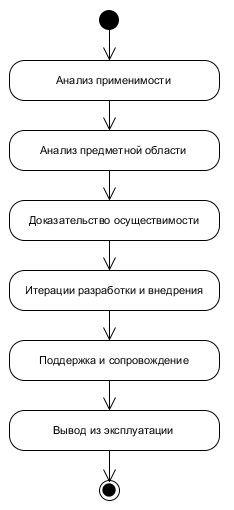
\includegraphics[width=0.35\textwidth]{part3/classicMethodology.png}
		\caption{<<Классическая>> методика разработки.}
		\label{classicMethodology}
	\end{center}
\end{wrapfigure}

\textbf{Глава 3} содержит описание предлагаемого подхода к разработке 
DSM-решений. Приводятся этапы жизненного цикла DSM-решения, обсуждается 
возможная степень автоматизации каждого этапа, формулируются требования к 
средствам автоматизации, приводится описание предлагаемой технологии. Предлагается
два варианта методик разработки --- <<Классическая>> методика и методика <<Метамоделирования
на лету>>, которая является вариантом классической и служит для упрощения первых этапов
жизненного цикла DSM-решения. Схематически <<Классическая>> методика изображена на рисунке
\ref{classicMethodology}.

Фаза разработки и внедрения состоит из нескольких итераций, порядок действий для каждой 
из которых представлен на рисунке~\ref{classicMethodologyIteration}. 

Такая методика называется классической, поскольку примерно такой схемы придерживается
большинство существующих DSM-платформ и большинство авторов, описывающих процесс создания
предметно-ориентированных языков и дающих рекомендации по этому процессу. Вклад данного 
исследования состоит в структуризации этапов жизненного цикла, описании действий на 
каждом этапе жизненного цикла и предложения технологии автоматизации каждого этапа.
Основная идея, предлагаемая здесь --- использование визуальных языков на каждом
этапе жизненного цикла, вплоть до описания генераторов.

С методологической точки зрения научную новизну имеет предлагаемый здесь подход 
<<Метамоделирования на лету>>. Ключевой принцип данной методики состоит в том, 
что создание визуального языка проходит непосредственно в процессе рисования диаграммы, 
без использования метаредактора.

\begin{figure} [ht]
	\begin{center}
		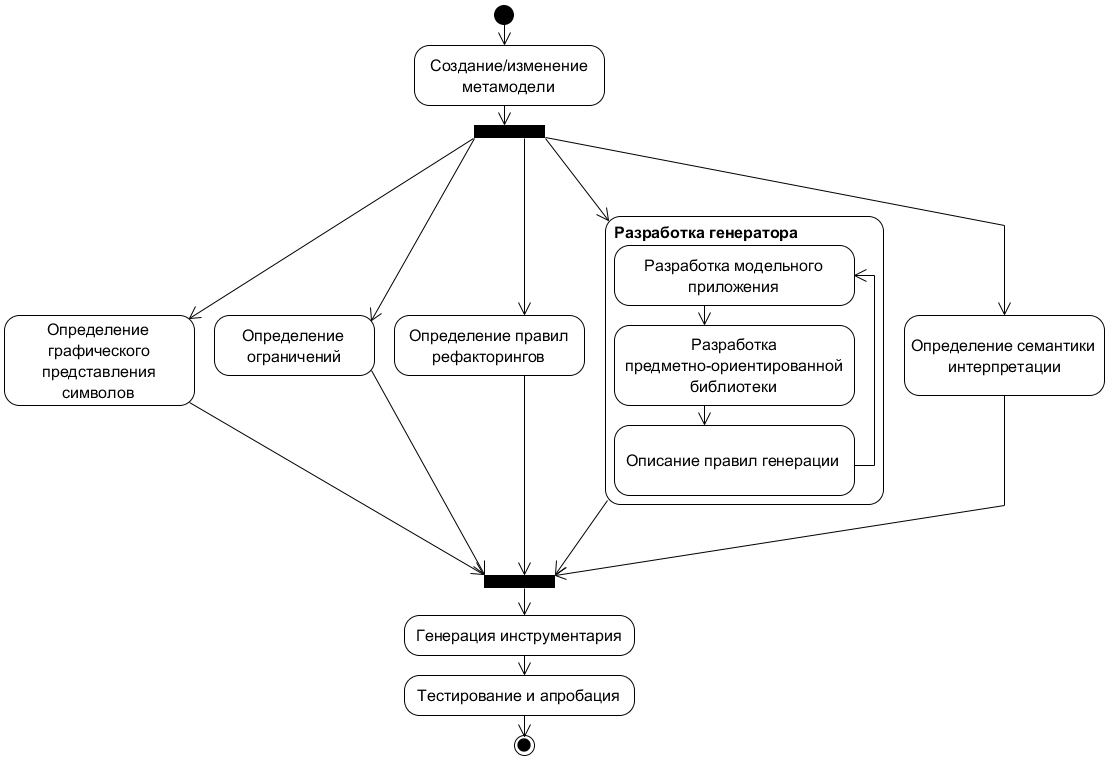
\includegraphics[width=1\textwidth]{part3/classicMethodologyIteration.png}
		\caption{Итерация проектирования и разработки языка.}
		\label{classicMethodologyIteration}
	\end{center}
\end{figure}

Основной этап предлагаемой методики --- прототипирование языка --- начинается сразу 
после этапа анализа применимости. Разработчик языка и будущий пользователь работают 
за одним рабочим местом. При запуске DSM-платформы они видят канву для рисования и 
пустую палитру. Пользователь объясняет, что он примерно хотел бы нарисовать, разработчик 
языка добавляет на палитру новые элементы, определяет для них графическое представление, 
пользователь рисует. Пользователь может сказать, что такой-то элемент должен содержать 
такую-то дополнительную информацию, тогда разработчик добавляет элементу новое свойство, 
задаёт его тип и значение по умолчанию, и пользователь продолжает рисовать диаграмму, 
используя новое свойство. Через некоторое время пользователь может сам добавлять и 
редактировать типы элементов, и работа полностью передаётся ему, разработчик языка 
лишь следит за процессом и консультирует при необходимости пользователя. Работа заканчивается, 
когда модельное приложение полностью нарисовано, после чего текущая интерпретируемая 
метамодель сохраняется в виде, пригодном для дальнейшего редактирования в метаредакторе. 
После этой фазы идут итерации <<классической>> методики по доработке созданного 
прототипа, дополнению его ограничениями, рефакторингами, интерпретатором и генератором, 
подготовке инсталляционного пакета, развертыванию и сбору обратной связи. На этих этапах 
пользователи, как и в <<классической>> модели, непосредственно в разработке не участвуют, 
поскольку этапы гораздо более продолжительны во времени и прямо при пользователе выполнены 
быть не могут.

\begin{wrapfigure}{R}{0.35\textwidth}
	\begin{center}
		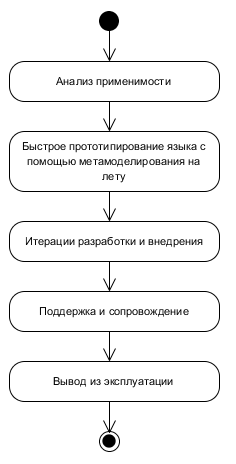
\includegraphics[width=0.35\textwidth]{part3/metamodelingOnFly.png}
		\caption{Методика <<метамоделирования на лету>>.}
		\label{metamodelingOnFly}
	\end{center}
\end{wrapfigure}

Модель жизненного цикла языка, использующая <<метамоделирование на лету>>, представлена 
на рисунке~\ref{metamodelingOnFly}.

В \textbf{главе 4} анализируются результаты реализации инструментальных средств поддержки предлагаемой 
технологии в проекте QReal. Описываются возможности системы QReal, связанные с поддержкой 
техник метамоделирования, включая метамоделирование на лету, принятые архитектурные 
решения. Также описывается эксперимент по сравнению трудозатрат на разработку инструментальных
средств поддержки визуального языка в QReal и в ведущих DSM-платформах. Эксперимент 
показал, что разработка в QReal требует меньших трудозатрат, это подтверждает достижение цели работы.

\textbf{Приложение A} содержит примеры применения результатов, описанных в данной 
диссертации, для разработки DSM-решений. Описывается среда QReal:Robots, то, какие 
преимущества были получены от использования DSM-платформы QReal при её разработке, 
то, чем QReal помочь не смог, и почему. Также приводится описание среды разработки 
сервисов для мобильных телефонов QReal:Ubiq и среды разработки аппаратуры QReal:HaSCoL, 
описываются их визуальные языки, достоинства и недостатки принятых при их создании подходов.

В \textbf{приложении B} описывается визуальный метаязык системы QReal.

В \textbf{приложении C} приводятся копии актов о внедрении результатов диссертационного исследования.

В \textbf{заключении} приведены итоги выполненного исследования, рекомендации и перспективы дальнейшего развития.

\subsection*{\Large Заключение}
\textbf{Итоги} диссертационной работы таковы.
\begin{enumerate}
	\item Разработана методика для создания предметно-ориентированных визуальных языков с помощью 
		визуального языка метамоделирования и других визуальных языков.
	\item Предложен новый способ метамоделирования: <<метамоделирование на лету>>, позволяющий
		доопределять и изменять визуальный язык в процессе его использования.
	\item Предложенные методики реализованы в виде технологии на базе системы QReal.
	\item Проведена апробация разработанных методик и технологии при создании инструментальных средств 
		среды программирования роботов QReal:Robots и других предметно-ориентированных решений.
\end{enumerate}
Были сформулированы следующие \textbf{рекомендации} по применению полученных результатов.
\begin{enumerate}
	\item Предложенные методики подходят для реализации небольших и средних по размерам 
		предметно-ориентированных языков.
	\item Наиболее эффективны предлагаемые методики в ситуации, когда нет чёткого представления
		о языке, который должен быть создан, но есть эксперт предметной области, участвующий
		в создании языка
\end{enumerate}
Также были сформулированы \textbf{перспективы дальнейшей работы}: реализация интеграции 
созданных инструментальных средств с существующими средствами других коллективов, 
проведение экспериментов по количественной оценке эффективности предложенных методик 
и средств в промышленных условиях и сравнению с существующими DSM-платформами, исследование 
применимости и возможных расширений предлагаемых методик для работы с большими предметно-ориентированными 
языками.






















